\documentclass[10pt,a4paper]{scrartcl}

\usepackage[utf8x]{inputenc}
\usepackage{ucs}
\usepackage{amsmath}
\usepackage{amsfonts}
\usepackage{amssymb}
%\usepackage{subfig}
\usepackage{graphicx}
\usepackage[british]{babel}
\usepackage{subfigure}

\setlength{\parskip}{0.5em}


\title{Sputnik}
\subtitle{Project Report HCC Project Seminar 2011}
\author{Simon Wallner\footnote{\texttt{me@simonwallner.at}}}

\begin{document}
\maketitle

\begin{abstract}
This paper evaluates \emph{Sputnik} a 3D environment with which the user can freely interact through an elastic \emph{arc of light/fishing rod} metaphor, to explore, create and interact with virtual \emph{sound objects}. These sound objects are placed in the scene and react to the user's input by sending MIDI commands to an external audio program thus creating or manipulating the sound.

\end{abstract}

\section{Reading Guide}
Appendices
Code
Prerequisitions
Video
CD
etc...


\section{Introduction}

% setting the scene
Computer music is around us for some time now and through the use of the computer musicians have sheer endless possibilities of musical expression. With this plethora of possibilities comes the need for constraints and control to harness this expressive potential. Over the recent years many standard and non-standard interface have been developed, ranging from the ordinary button-fader-nob MIDI interface to more elaborate interfaces and systems like the \emph{reactable}\cite{Jorda2007}, \emph{mixiTUI}\cite{Pedersen2009} or commercial solutions like the \emph{Novation Launchpad}\footnote{\texttt{http://www.novationmusic.com/products/midi\_controllers/launchpad}} or \emph{Native Instruments Maschine}\footnote{\texttt{http://www.native-instruments.com/\#/en/products/producer/maschine/}} to name but a few.

With the advent of motion based controllers in consumer entertainment systems, marked by the release of the \emph{Wii}\footnote{\texttt{http://de.wikipedia.org/wiki/Wii}} console in late 2006, motion controllers became widely and cheaply available. This and their interface capabilities make them the ideal tools to explore the realm of \emph{new interfaces for musical expression}.


% problem statement
A common problem of computer music interfaces is that often the process of sound creation is not readily comprehensible. Seeing a performer on stage behind their laptop twisting knobs and adjusting faders might be ambiguous to an uninformed observer. It can be hard to relate the artist's action to the resulting sounds. This can hinder the experience and might go as far as to the point where the audience suspects that an artist just pressed play, as interviews conducted by \cite{Pedersen2009} show.

% Sputnik description
This paper introduces \emph{Sputnik}, a system that uses a \emph{Wiimote} controller to interact with a dynamic 3D scene. In the scene, a variety of sound creating objects are placed that send MIDI signals to an external audio program upon the user's interaction. 

Users can freely navigate the 3D scene and interact with it through an elastic \emph{arc of light/fishing rod} metaphor. It seems as if the \emph{arc of light} was coming out of the Wiimote and reaches into the scene, acting as an extension of the user's body into the virtual space. With this bodily extension users can \emph{grab} and \emph{drag} objects around the 3D scene.



% contribution
In this paper I evaluate the qualities of the \emph{arc or light} metaphor and how the design decisions/constraints of the system influence its expressive potential both visually and musically. This evaluation is grounded in a user study of XXX users.

Based on these findings and the theoretical framework of \cite{Ullmer2000} the similarities and differences between \emph{Sputnik} and tangible user interfaces are discussed. 


\section{Paper Outline}
The following section gives an overview over related work in the field of \emph{New Interfaces for Musical Expression} and tangible user interfaces. Section \ref{sec:results} goes into detail about Sputnik, both on a conceptual and a technical level. Section \ref{sec:evaluation} describes the performed user study and the paper is finally concluded in section \ref{sec:discussion} where the findings are discussed.


\section{Related Work}
\paragraph{Practical Work}
Only a few projects exist that go into a similar direction as Sputnik. The \emph{Virtual Xylophone}\cite{Maki-Patola2005} is a virtual reality system in which the user can place xylophone bars of different pitch in the scene and then struck them with a virtual mallet. By translating the configuration and mapping of the real instrument into the VR environment, new modes of play emerge.
\cite{Zappi2010} created a virtual controller for \emph{Ableton Live} that allows users to create simple proxy objects in a VR environment, bind them to certain controls and use them effectively as virtual sliders. \cite{Rodet2005} created a virtual environment for an exhibition setting. Users interact with the system via a 6-DOF motion tracker with tactile feedback. However, the user's actions in the system are highly constrained.

More projects can be found in the realm of Tangible User Interfaces. With \emph{mixiTUI} \cite{Pedersen2009} created a table top tangible interface for a sequencer that aimed not only to be functional but also to visually enrich the artists performance. Interviews with musicians and an extensive user study have been performed. \cite{Jorda2007} created the famous \emph{reacTable}, also a table top tangible interface that allows the creation and manipulation of music by composing various objects on its surface. 

After the release of the Wii in late 2006, the Wiimote motion controller received some attention in and outside the field of musical interfaces: 
\cite{Kiefer2008} assess the general qualities of the Wiimote as a musical controller and \cite{Miller2010} uses the Wiimote and sensor bar to create the \emph{Wiiolin}, a virtual violin that mimics the real instrument and can be played either in an upright position like a cello or horizontally like a violin. It senses the button presses and tracks the movement of the \emph{bow}, i.e. the sensor bar to create the sounds.

Not a Wiimote but still impressive, \cite{Miyama2010} uses an low resolution distance sensor array to control the many parameters of a synthesizer. A small gui application is merely used for monitoring the system's state, and sound creation is done in pd.


\paragraph{Theoretical Work}
The field of \emph{Tangible User Interfaces (TUI)} provides part of the theoretical background for this work. Work of \cite{Fitzmaurice1995} and then later \cite{Ishii1997} introduced this term and the wider concept. \cite{Shaer2009} Gives a very good overview over this field as well as the history of TUI studies. \cite{Ullmer2000} introduced \emph{MCRpd}, a formal model for describing and analysing TUIs that will be used in section \ref{}.

\cite{Sharlin2004} introduced \emph{spacial TUIs} that focuses on \emph{I/O unification} by tightly coupling the action and perception spaces and embodying a clear state representation across all sensory modalities.


Entering the musical realm \cite{Fels2011} give a good overview and general introduction into the field of \emph{NIMEs (New Interfaces for Musical Expression)}. \cite{Cook2001} shares 13 general principles for designing computer music controllers that resulted from his long lasting experience in this field. \cite{Dobrian2006} asks the question of virtuosity and expression by pointing out the elephant in the room, e.g. the lack thereof and also the lack of a comparable standard repertoire. 

In contrary to that \cite{Gurevich2007} question the hegemonic \emph{composer--interpret--listener} relation in favour of a more holistic \emph{ecological} view of musical expression. Later work by \cite{Gurevich2010} evaluated a highly constrained, prototypical one-button instrument that spurred a wide variety of play styles in test users.

Closing the loop to design and HCI, \cite{Magnusson2010} gives a good overview over the field of \emph{affordance} and elaborates on \emph{contraints} from different viewing angles and how they impact and support creativity. Finally, \cite{Wanderley2002} goes into depth over evaluating input devices for musical expression in the context of HCI. 






% ------------------------------------------------

% \cite{Magnusson2010} gives a good overview over the field of \emph{affordance} and elaborates on \emph{constraints} from different viewing anlges and how constraints impact and support creativity.

% \cite{Ullmer2000} introduces a formal model for tangible user interfaces and compares it to the prevalent MVC (Model View Controller) model. Different qualities of TUIs are stated and a few existing applications are assessed with it.

% \cite{Ishii1997} Introduced the term \emph{Tangible User Interface} (\emph{TUI}

% \cite{Kiefer2008} Assessing the potential of the wiimote as an musical interface and comparing it to a common interface. user study, only very simple mapping + perceptron shape recognition

% \cite{Wanderley2002} discusses the problems of how to assess interfaces for musical expression and searches the depths of HCI studies for a possible answer. no answer given

% \cite{Dobrian2006} tries to answer what constitutes an expressive musical interface, and how does the lack of virtuoso performers impacts the whole discussion. It highlights the role of a repertoire and the role of the performer. This is a bit contradicting to what \cite{Magnusson2010} writes.

% \cite{Cook2001} provides a few (empiric) design principles for digital musical instruments and richly illustrates them with example projects.

% \cite{Fels2011} General introduction and overview to/of the field of NIMEs given as a SIGGRAPH course. The definitive introduction to NIMEs.

% \cite{Gurevich2007} introduce an \emph{ecological} view of musical expression that goes against the conservative view of a uni-linear composer--interpret--listener relation.

% \cite{Gurevich2010} evaluate a highly constrainted one-button instrument in terms of the style and variations these constraints induce.

% \cite{Maki-Patola2005} built four virtual reality instruments for a cave like environment, one of them being a virtual mallet, where users can hit the pads with virtual mallets. This comes closest to Sputnik and also a few general thought on virtual scenes and the possible impact on the performance are given.

% \cite{Miller2010} uses the Wiimote and sensor bar to modell a virtual violin. It has no graphical UI and uses recorded sound samples.

% \cite{Miyama2010} IR distance sensor array used to control a pd patch and a simple gui application written in c.

% \cite{Pedersen2009} mixiTUI, tangible sequencer with gui, user study and interviews.

% \cite{Sharlin2004} introduces \emph{spatial TUIs} and discusses I/O unification on a few examples, coupling of action and perception space.

% \cite{Fitzmaurice1995} introduces \emph{graspable user interfaces} with Briks.

% not used
% \cite{Gamberini2011} introduces \emph{action breakdowns} for quantitative studies of user interfaces.

% \cite{Shaer2009} Give a general introduction into the field of TUIs and provide an historical overview.

% furhter research
% \cite{Godoey2006} explores the the playing of \emph{air instruments} and what is behind it. 

% \cite{Zappi2010} built a motion tracked 3d virtual environment in which users can create/bind/interact with basic virtual objects to control all aspects of a \emph{live} set. Input done via hand gestures only simple parameter mapping, virtual faders.

% \cite{Rodet2005} haptic feedback to objects in a ve, very simple interaction, no direct scene interaction.






% results

% Create a system that allows the user to interact with an virtual world through the Wiimote. This system should be intuitive even for untrained users, and have a very low barrier of entry.
% Explore the technical capabilities of the Wiimote and Nunchuck controller and put it to good use.
% Create a meaningful mapping form the virtual world to the sound generation system.
% Create a sound generation system that allows nuanced and rich musical expression.
% Develop an architecture that streamlines the three stages input - processing - output.


\section{Sputnik Overview}
% user domain description of Sputnik
% what is Sputnik in the user domain. Everything that is not technical or theoretical. This sets up the frame for alle the following section.

\emph{Sputnik} is a \emph{New Interface for Musical Expression} that combines 3D graphics with the capabilities of the Wiimote controller. The user is presented with colourful 3D scene that contains various simple objects. The user can freely navigate this scene and interact with these object to create sounds.

The user can interact with the system via a Wiimote and Nunchuck controller. The Nunchuck controls the users movement in the 3D space and the Wiimote is used to control the camera and to interact with the objects in the scene. 

\subsection{Setup}
The system is set up in a room with an overhead mounted video beamer. The sensor bar can either be placed on the upper or lower edge of the projected image. It consists of two IR emitters that allows the IR camera in the Wiimote to track its relative orientation in space. A Wiimote and Nunchuck controller are used and only a single person at a time can use the system. Figure \ref{fig:sputnik-setup} illustrates the setup.

\begin{figure}[hbtp]
\begin{center}
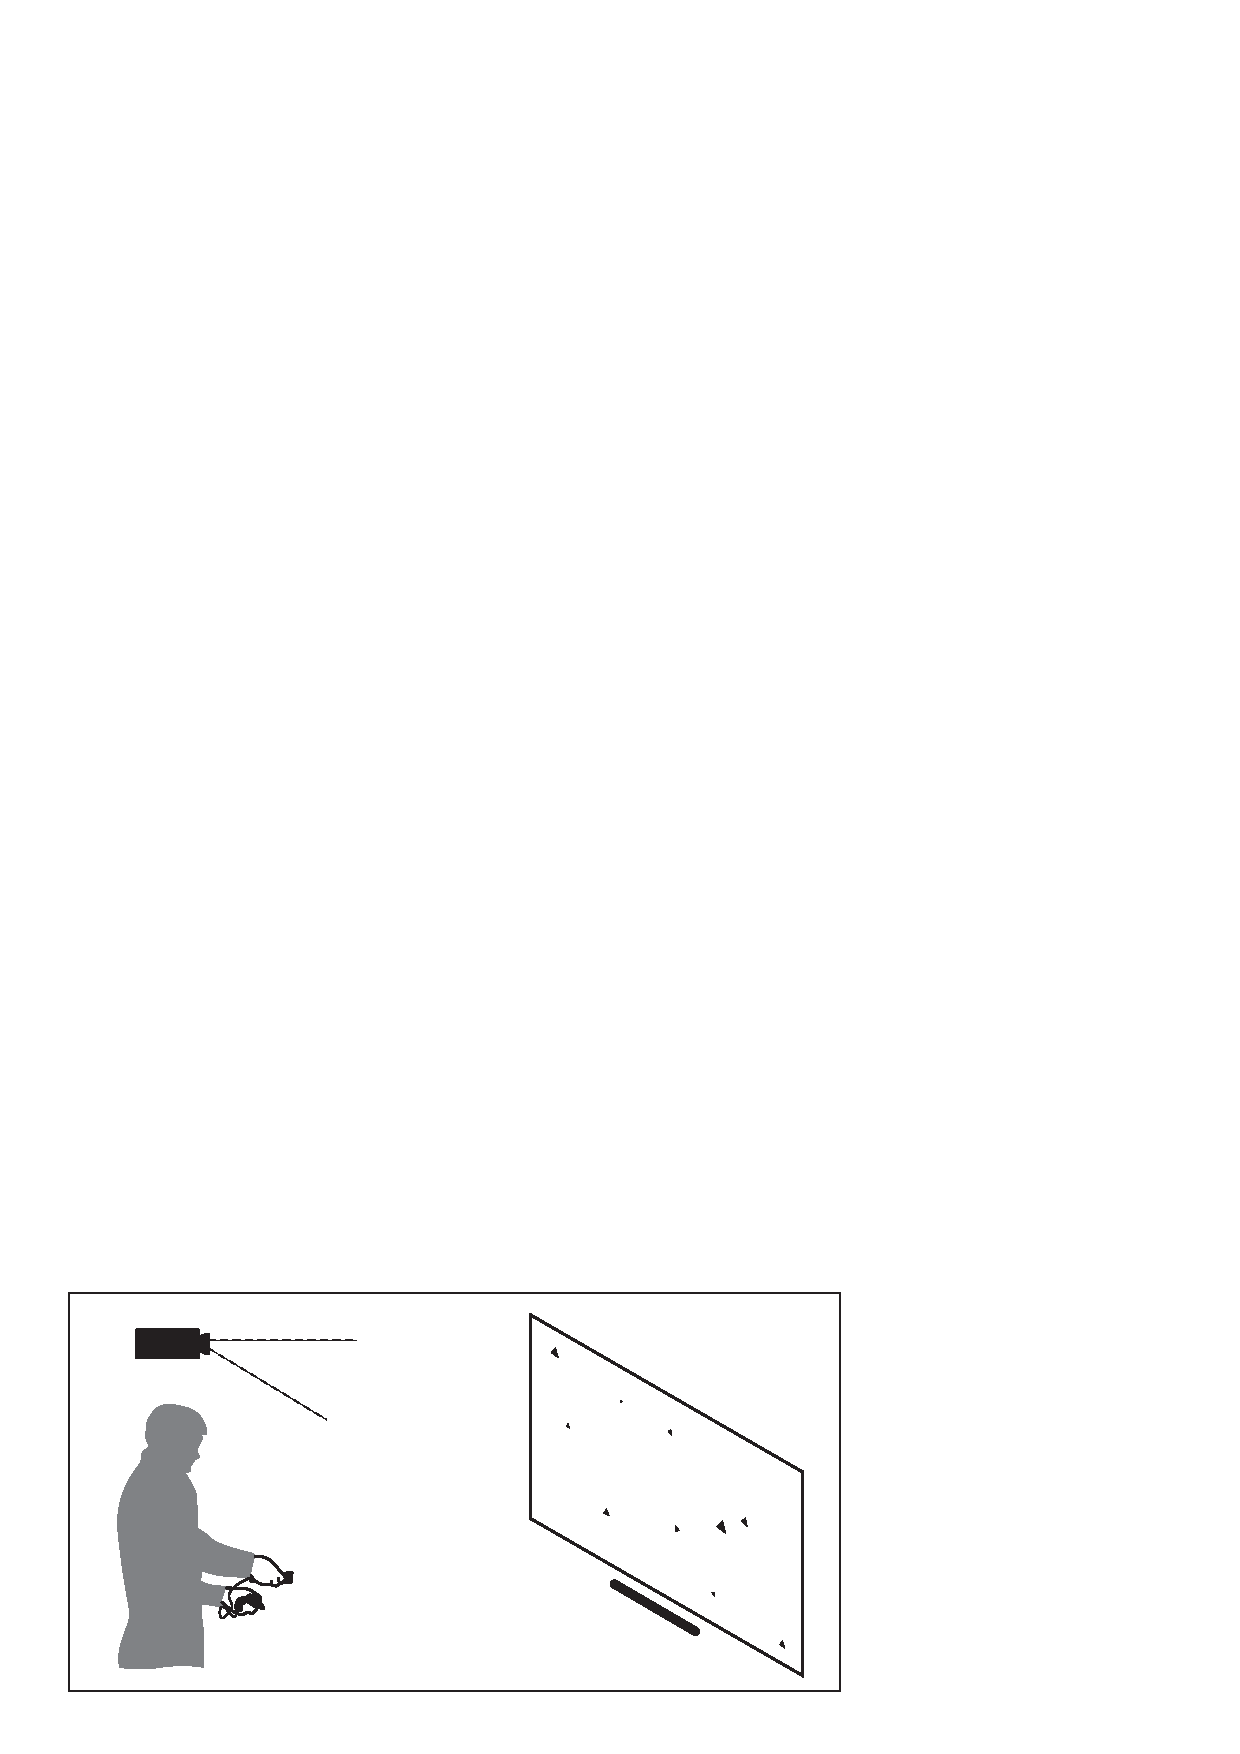
\includegraphics[width=0.4\columnwidth]{img/setup}
\caption{Standard set up of Sputnik}
\label{fig:sputnik-setup}
\end{center}
\end{figure}



\subsection{Navigation and Camera Controls}
Sputnik's virtual scene uses a fixed \emph{up direction} and the user can move through the scene by pushing the Nunchuck's analogue stick in the respective direction. Pushing the stick forward moves the camera into the scene, pushing it left moves the camera to the left and vice versa.

Tilting and panning is controlled by pointing the Wiimote to the top/bottom/left/right of the screen. The farther it is pointed away from the neutral center position the faster the camera movement is. Figure \ref{fig:sputnik-navigation} illustrates the navigation.

\begin{figure}[hbtp]
\begin{center}
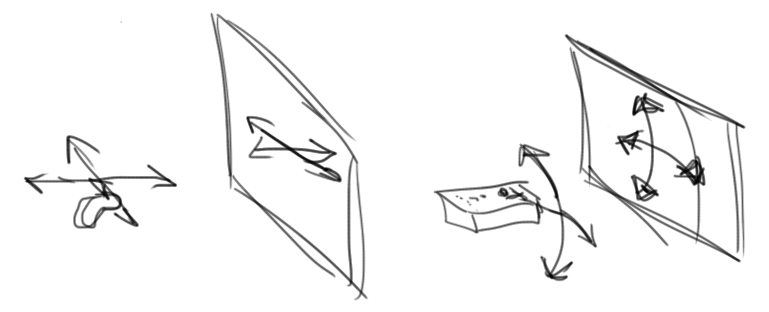
\includegraphics[width=0.7\columnwidth]{img/navigation}
\caption{The Nunchuk's analogue stick controls the camera's dolly and track movements, the Wiimote's IR pointer controls the camera's tilt and pan movements.}
\label{fig:sputnik-navigation}
\end{center}
\end{figure}




\subsection{Interaction}

\begin{figure}[hbtp]
\begin{center}
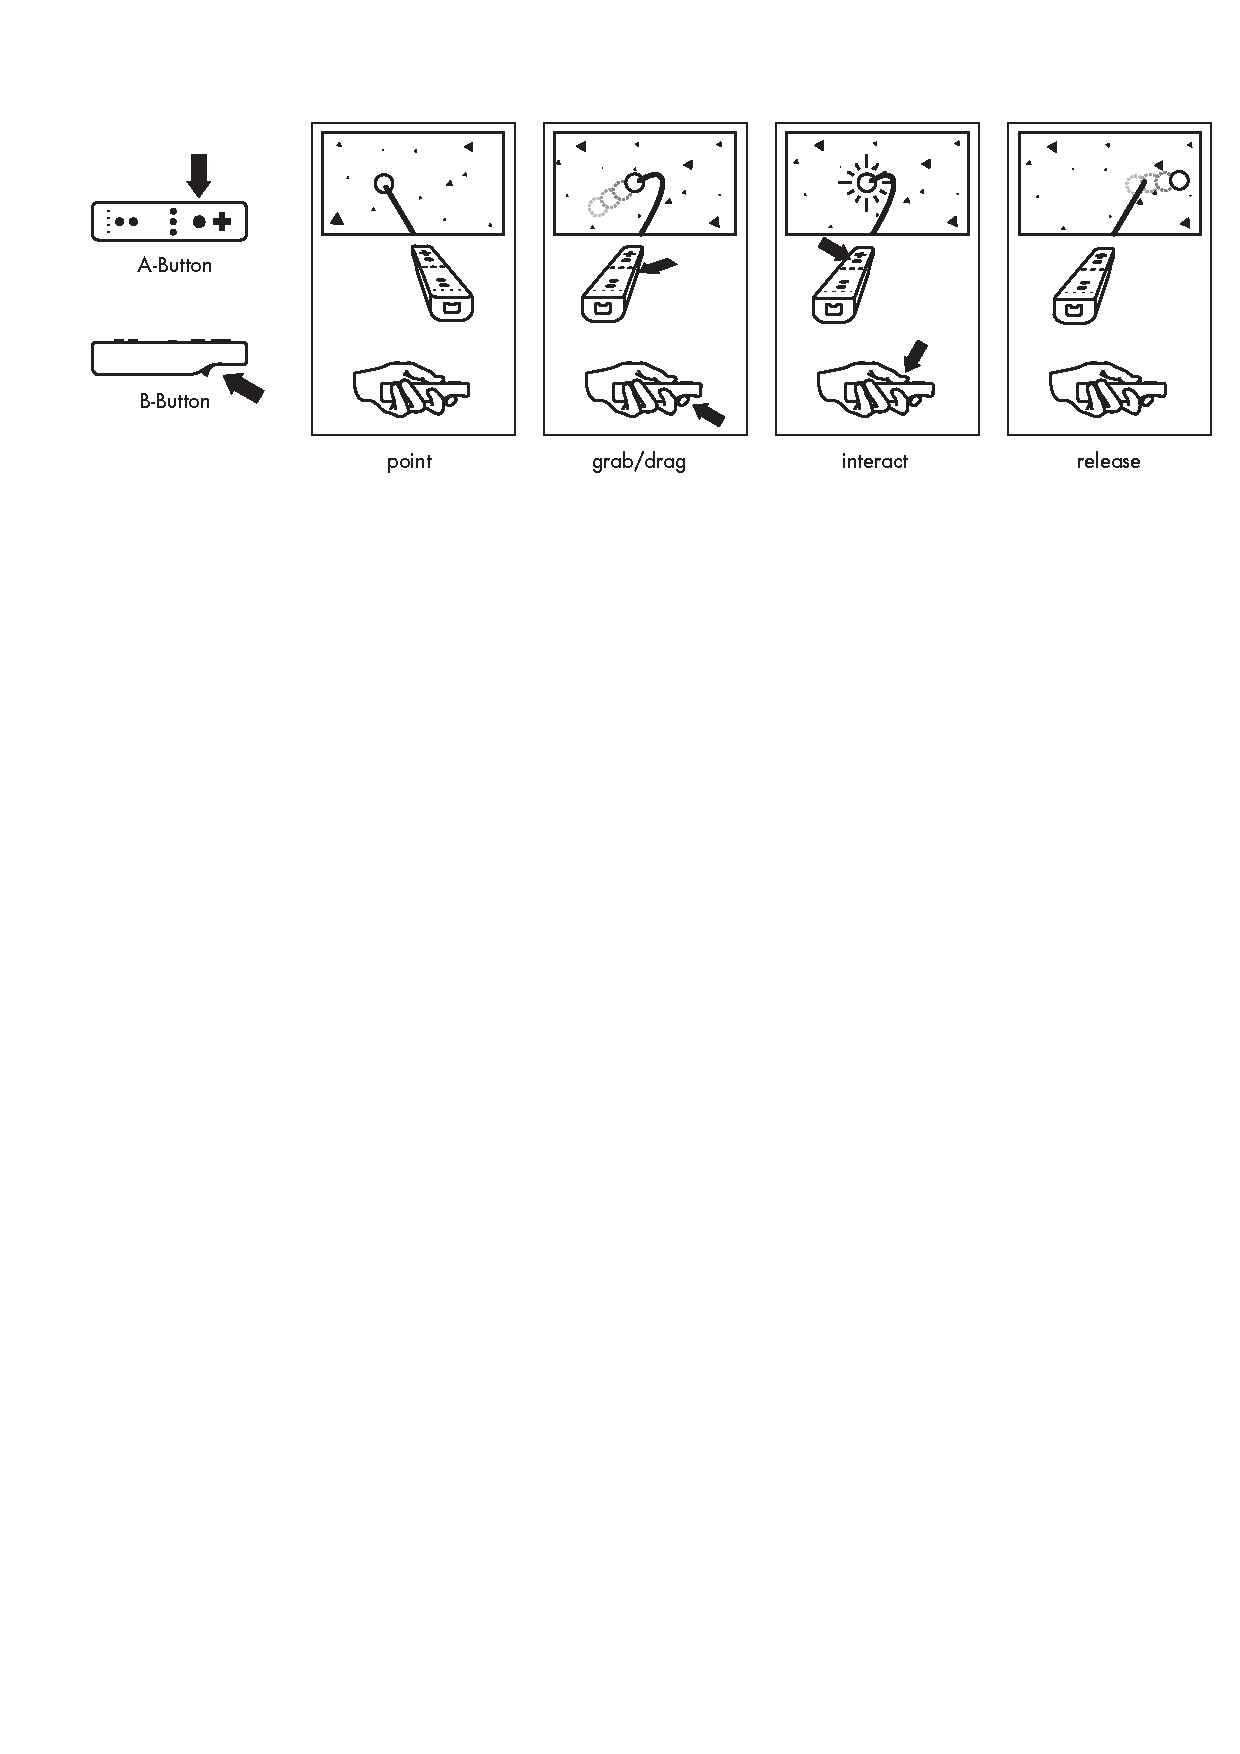
\includegraphics[width=0.95\columnwidth]{img/sputnik-overview}
\caption{The basic interaction vocabulary of Sputnik}
\label{fig:sputnik-overview}
\end{center}
\end{figure}

Figure \ref{fig:sputnik-overview} illustrates the basic interaction vocabulary of Sputnik. The user can interact with the scene via an \emph{arc of light} metaphor. It seems as if the arc of light was coming out of the Wiimote and reaches into the scene, acting as a bodily extension of the user into the virtual space. Through this \emph{arc} objects in the scene can be \emph{pointed} at, \emph{grabbed} and \emph{dragged} around.

Objects behave in a simplified yet physically plausible way, each featuring distinct weight and friction. Dragging objects causes the arc to bend like a fishing rod, reflecting the physical properties of the object.

Each object in the scene can react individually to user interaction. The following classes of objects exist in Sputnik:
\begin{description}
\item[Sampler (red sphere)] The \emph{sampler} object reacts to the press of the \emph{A Button} while it is grabbed. While the button is held the sample is played in a loop and stops immediately when the button or the object is released. Playback always starts at the beginning of the sample.

\item[Player (yellow sphere)] The \emph{player} object reacts to the press of the \emph{A Button} while it is grabbed. Pressing the \emph{A button} starts and stops the player. It is not automatically stopped when it is released. Playback is looped and always starts at the beginning.

\item[Tape Machine (grey sphere)] Modelled after an old tape machine and inspired by \emph{musique concrète} the \emph{tape machine} object controls the speed of the play back by the object's movement speed in the virtual space. The faster it moves the faster the playback. Playback is looped.

\item[Harmonic Harp (orange spheres)] The orange spheres form a kind kind \emph{harmonic harp}. Each sphere controls a single sine wave oscillator and the volume is determined by the the spheres distance to is origin. Additionally a force exists that drags the spheres towards their respective origins. The oscillators are tuned to the natural harmonic series.
\end{description}

By interacting with the different objects and arranging the in the virtual scene users can create musical performances that are both musically and visually expressive.


\subsection{The Arc Of Light Metaphor}
The \emph{arc of light} is the core of Sputnik. It should be easy to pick up and understand even for novice users. It has the following properties:

If no object is grabbed, the \emph{arc} follows the input of the user directly. The input is not filtered by the application and is used \emph{as is}. This creates a slight jittering but on the other hand makes it very responsive. Low pass filtering of the Wiimote input was explicitly not used in order to achieve high responsiveness.

This filtering however is indirectly introduced through the physical properties of the interactive objects. Giving this filter process a physical representation should it ideally make it transparent to the user and achieve the desired effect (even very strong filtering) without making the system feel laggy or dull.


\subsection{Simplified Physics}
Sputnik uses simplified physics simulations to give the interactive objects their distinct physical properties. An objects properties are described by \emph{mass}, a \emph{movement vector}, as well as a movement \emph{damping constant}. SI units are used unless otherwise noted.

The dragging force of the arc on an object is linear in the distance from the object to the intersection of the unbended arc with the plane that goes through the object with a plane normal pointing at the camera.

In each frame, the speed of an object is then computed as 
\begin{equation}
v_i = v_{i-1} + \frac{F * \Delta T}{m} 
\end{equation}
where $v_i$ is the object's movement vector in frame $i$, $F$ is the current force, $m$ is the mass and $\Delta T$ is the frame time. Force is only applied at the center of the objects, and thus never causes a rotation of the object.

Damping of objects movement is implemented by a simple exponential decay, given as
\begin{equation}
v_i = v_{i-1} * e^{-\lambda * \Delta T}
\end{equation}
where $\lambda$ is the damping constant.

Even with theses simple formulas a convincing and plausible physical system can be created. 


\subsection{Creating sound}
Sputnik's interactive objects use the MIDI  protocol to communicate with external applications. Thanks to the simplicity and the pervasiveness of this protocol, virtually every music software can be used together Sputnik. 

In the current set up Sputnik \emph{pure data (pd)}\footnote{\texttt{http://puredata.info/}} is used to create sound. A simple patch is used that builds on \emph{boctok-1}, a small collection of pd patches written by the author prior to this project. 



\section{Implementation}
Sputnik is implemented in C++ with Mac OS X as its development platform. The project is split into two sub projects: The special purpose Sputnik and the more general purpose \emph{kocmoc-core}. Kocmoc-core provides a host of core services that are then used by sputnik to build the final system. Some code of kocmoc-core existed prior to this project, but most of it was created during this project. 

The source code of of both Sputnik and kocmoc-core is licensed under the MIT license and is available to the public on github\footnote{\texttt{https://github.com/SimonWallner/sputnik}} \footnote{\texttt{https://github.com/SimonWallner/kocmoc-core}}.

Sputnik uses OpenGL 2.1 with a few extensions to display the virtual scene. The renderer is fairly simple and displays unlit, textured objects with baked ambient occlusion maps. A simplified physically correct computation of the homogeneous fog is realised in the vertex and fragment shader and a post processing effect is applied. This effect adds a barrel distortion and vignetting as well as a simple form of full screen anti aliasing.

The \emph{Assimp}\footnote{\texttt{http://assimp.sourceforge.net/}} and \emph{devIL}\footnote{\texttt{http://openil.sourceforge.net/}} libraries are used to load assets and font rendering is implemented using the \emph{freetype}\footnote{\texttt{http://www.freetype.org/}} library.

\emph{RtMidi}\footnote{\texttt{http://www.music.mcgill.ca/~gary/rtmidi/}} is used to send messages to external applications and \emph{WiiC}\footnote{\texttt{http://wiic.sourceforge.net/}} was used to interface with the Wiimote and Nunchuck controller.

Figure \ref{fig:flow} illustrates the data flow in the main run-loop. First the devices are polled, which causes callbacks to be fired. The components are subsequently updated and finally the scene is sent to the renderer.


\begin{figure}[hbtp]
\begin{center}
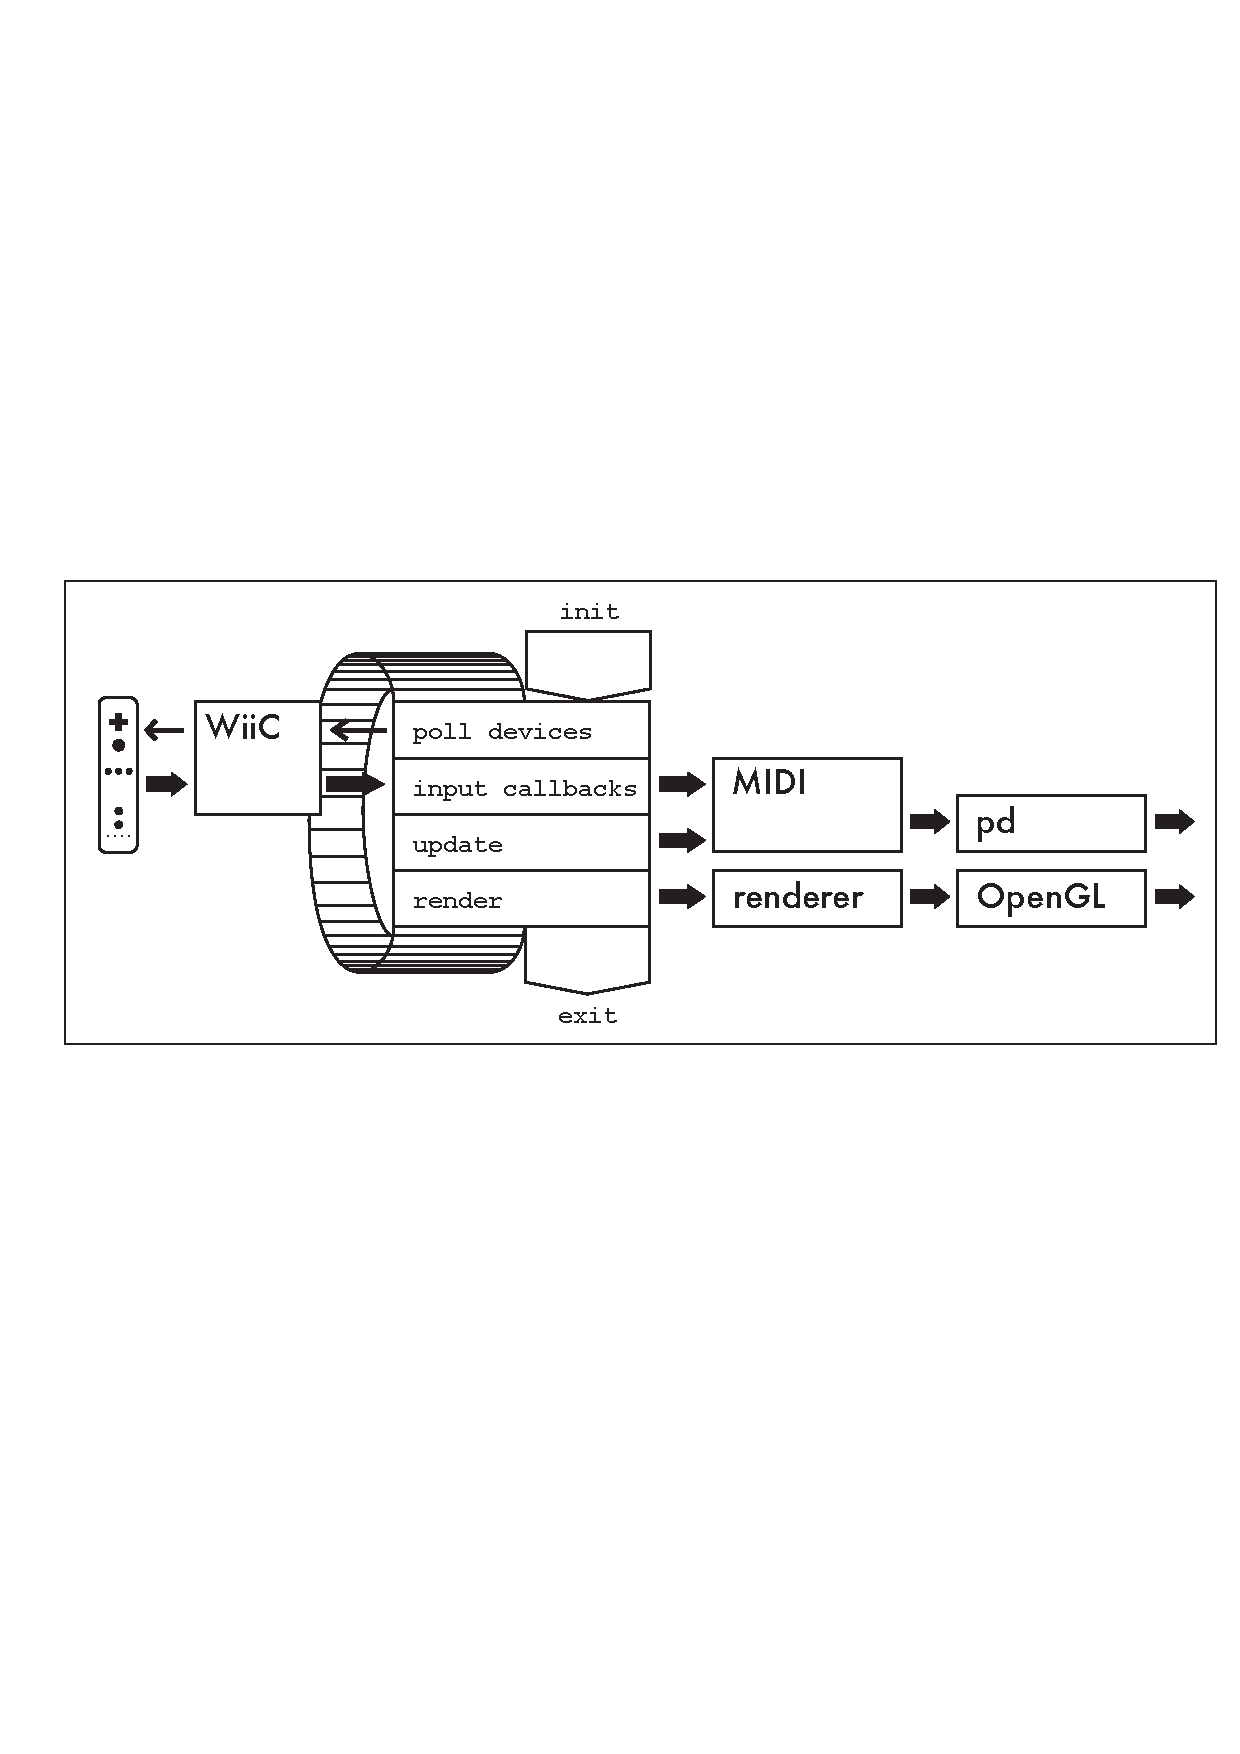
\includegraphics[width = 0.95 \columnwidth]{img/flow}
\caption{The data flow in the run-loop.}
\label{fig:flow}
\end{center}
\end{figure}



\subsection{The Virtual Scene}

\begin{figure}[hbtp]
\begin{center}
\subfigure{
	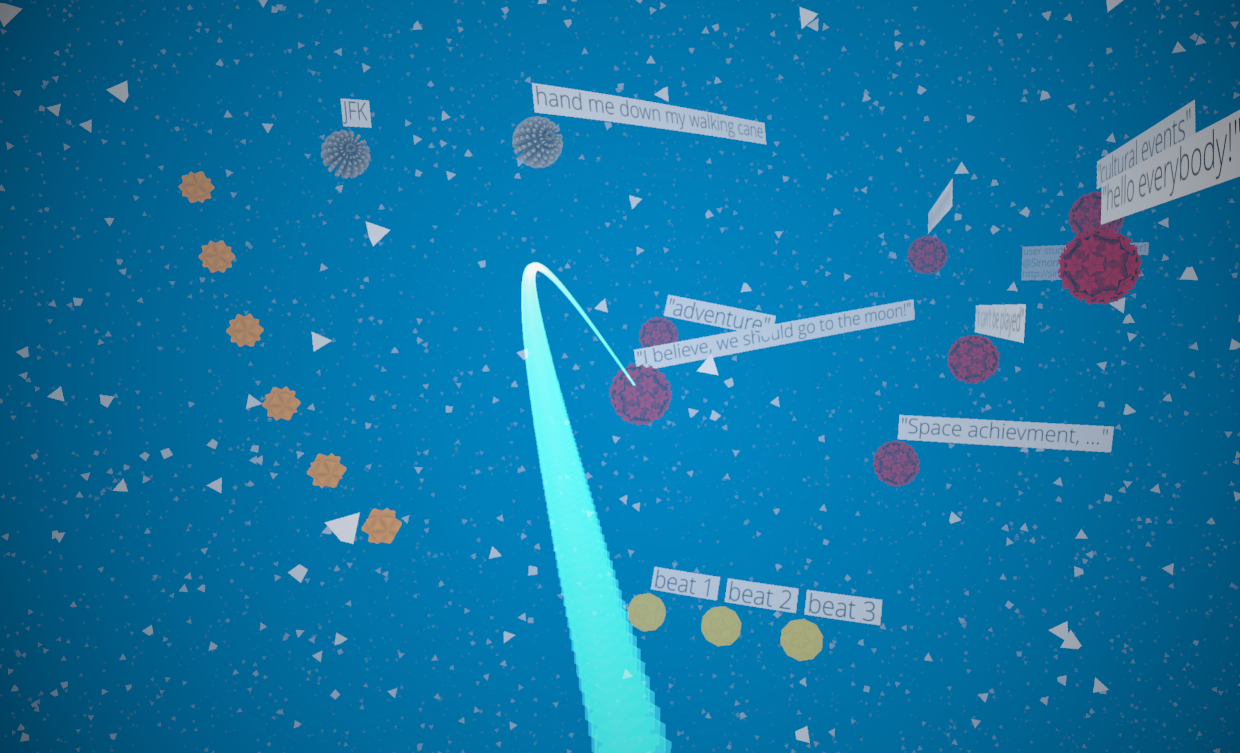
\includegraphics[width = 0.45\columnwidth]{img/screen-shot-all}
	\label{fig:screen-shot-overview}
}
\subfigure{
	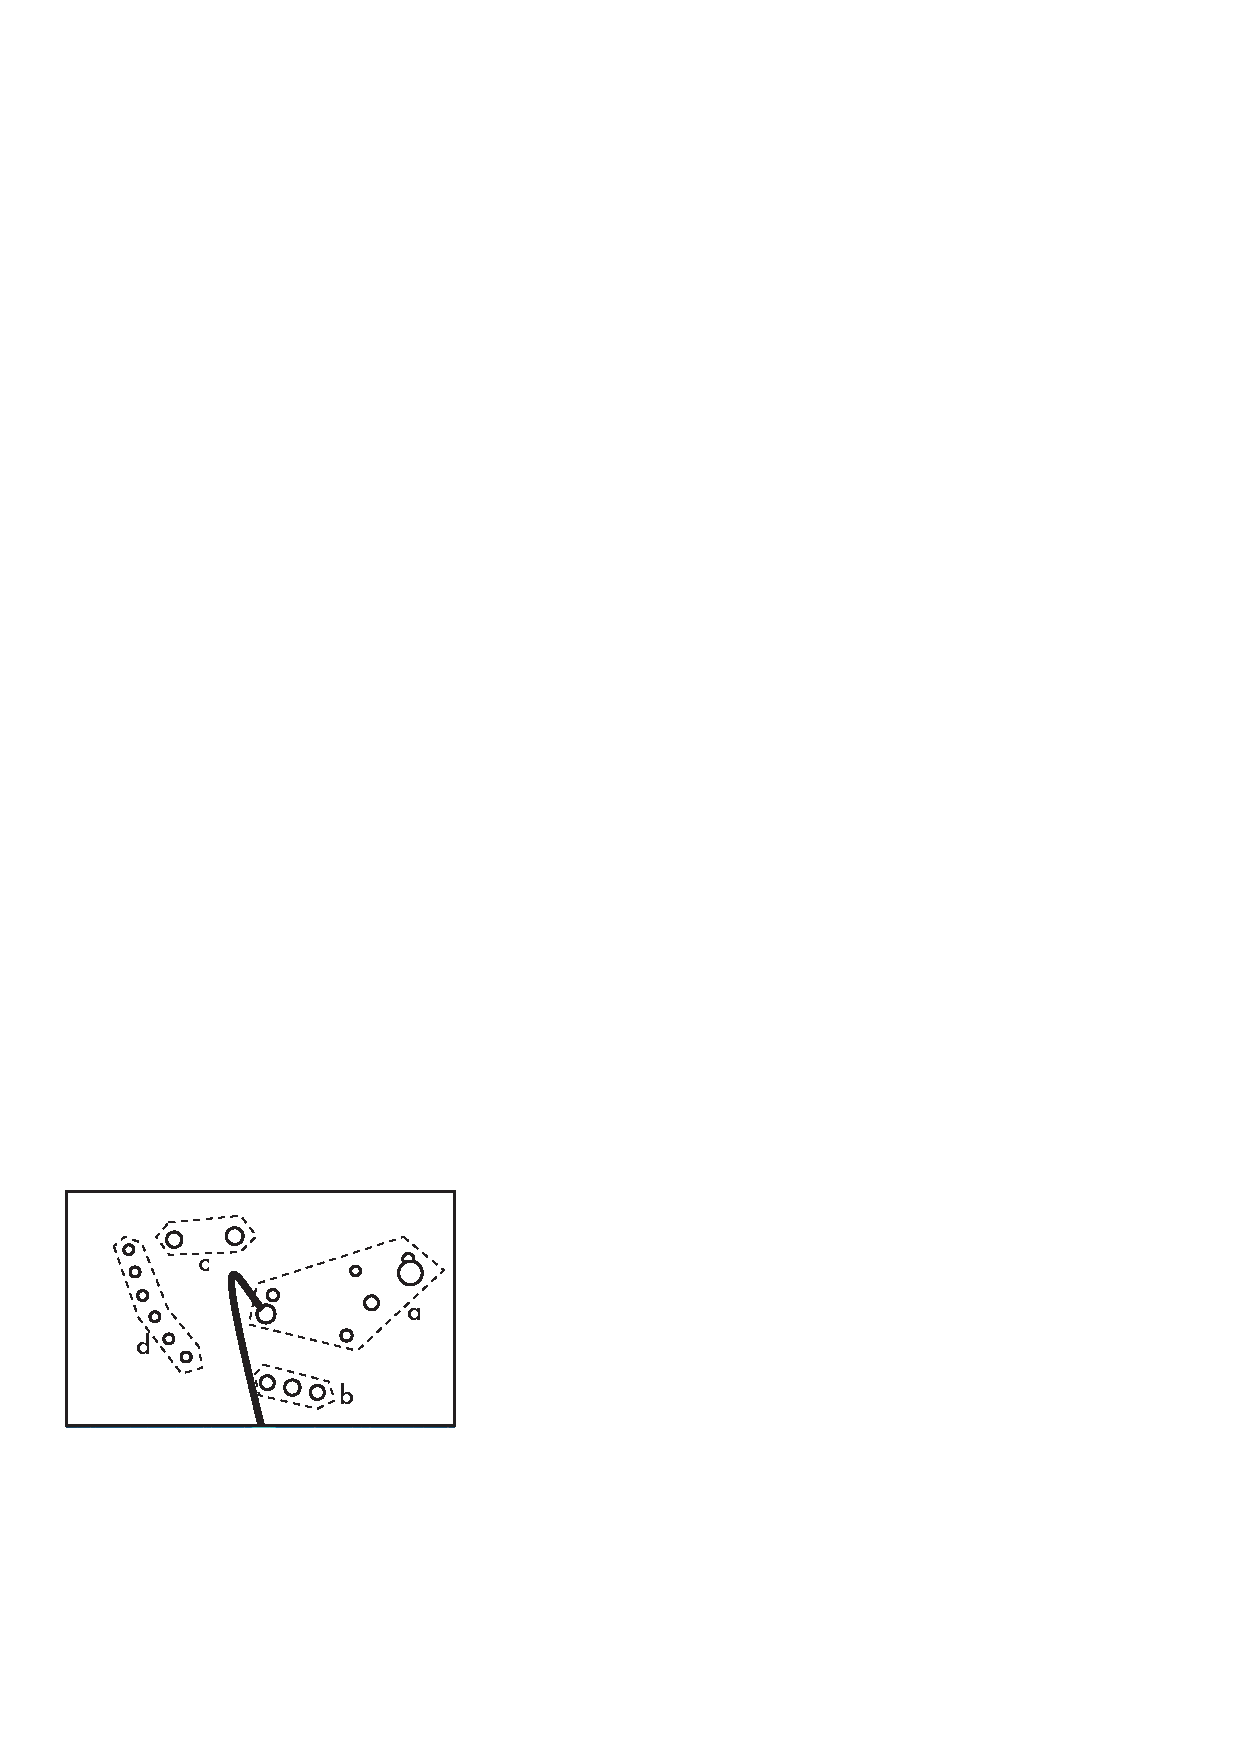
\includegraphics[width = 0.45 \columnwidth]{img/overview-illu}
}
\caption{The objects in the scene: (a) Samplers, (b) Players, (c) Tape Machines, (d) Harmonic Harp}
\end{center}
\end{figure}


Figure \ref{fig:screen-shot-overview} shows an overview shot of sputnik. The scene consists of the following parts:
\begin{enumerate}
\item The light blue and bent \emph{arc of light} starting in the middle of the lower edge and going \emph{into} the picture
\item Musical objects the user can interact with: sampler (red), player (yellow), tape machine (grey), harmonic harp (orange)
\item Textual Labels on the musical objects. These help the performer as well as they convey meaning to the audience.
\item The star field. It is randomly generated and the user cannot interact with it. It serves an aesthetic  purpose as well as it is an important orientation help. (see section \ref{})
\item The coloured fog. The fog provides an important depth cue to the human perception. 
\end{enumerate}


The visual representation of Sputnik serves a dual purpose. It it the sole graphical interface to the performer and thus has to display all relevant information that is needed for the performance but at the same time has to be visually pleasing to the audience. Common music software only focuses on the first, leaving the visual performance in most cases to a dedicated VJ. Sputnik tries to bridge those two areas by using the same interface for both the performer as well as the audience.

The textual labels play an important role in Sputnik. On the one hand they provide important information to the performer and on the other hand they act as an additional communication channel to the audience. The audience can read the labels and better understand what is happening and how the musical performance is built up from smaller building blocks. It can also introduce an element of anticipation when an object with a certain label is visible but the performer does not yet interact with it.


\begin{figure}[hbtp]
\begin{center}
\subfigure[]{
	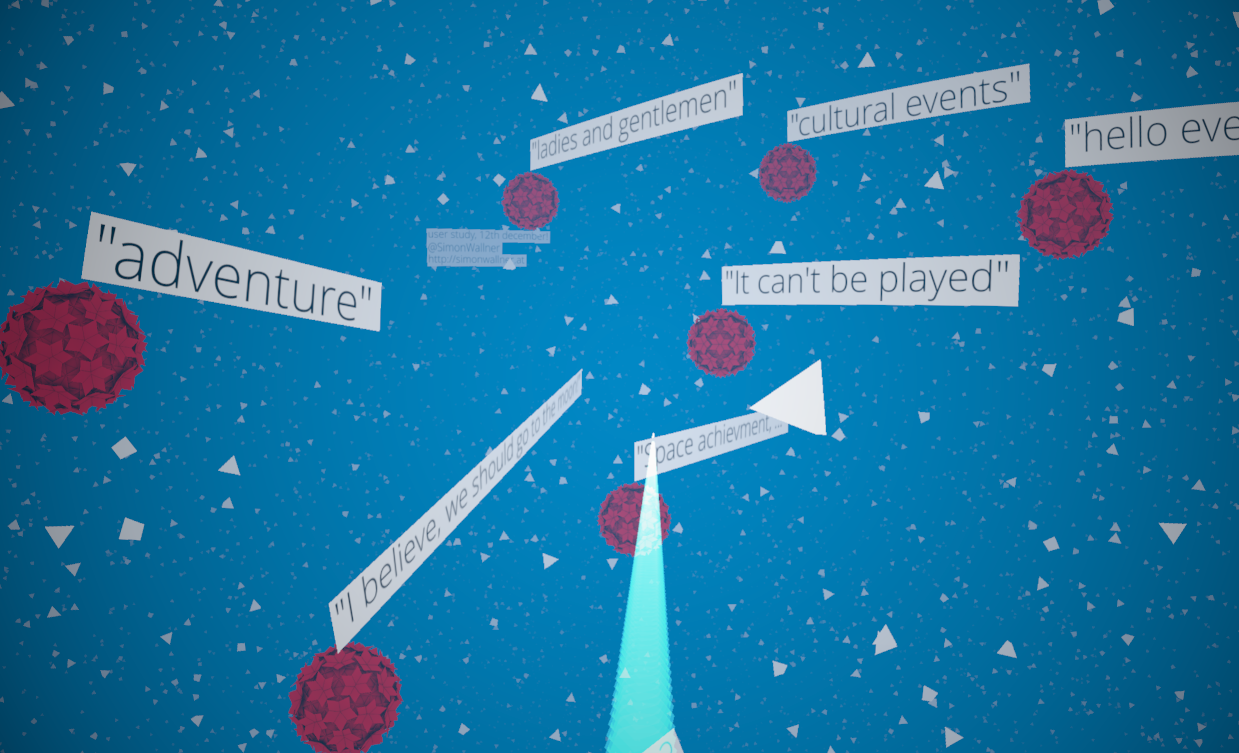
\includegraphics[width = 0.45\columnwidth]{img/screen-shot-sampler}
}
\subfigure[]{
	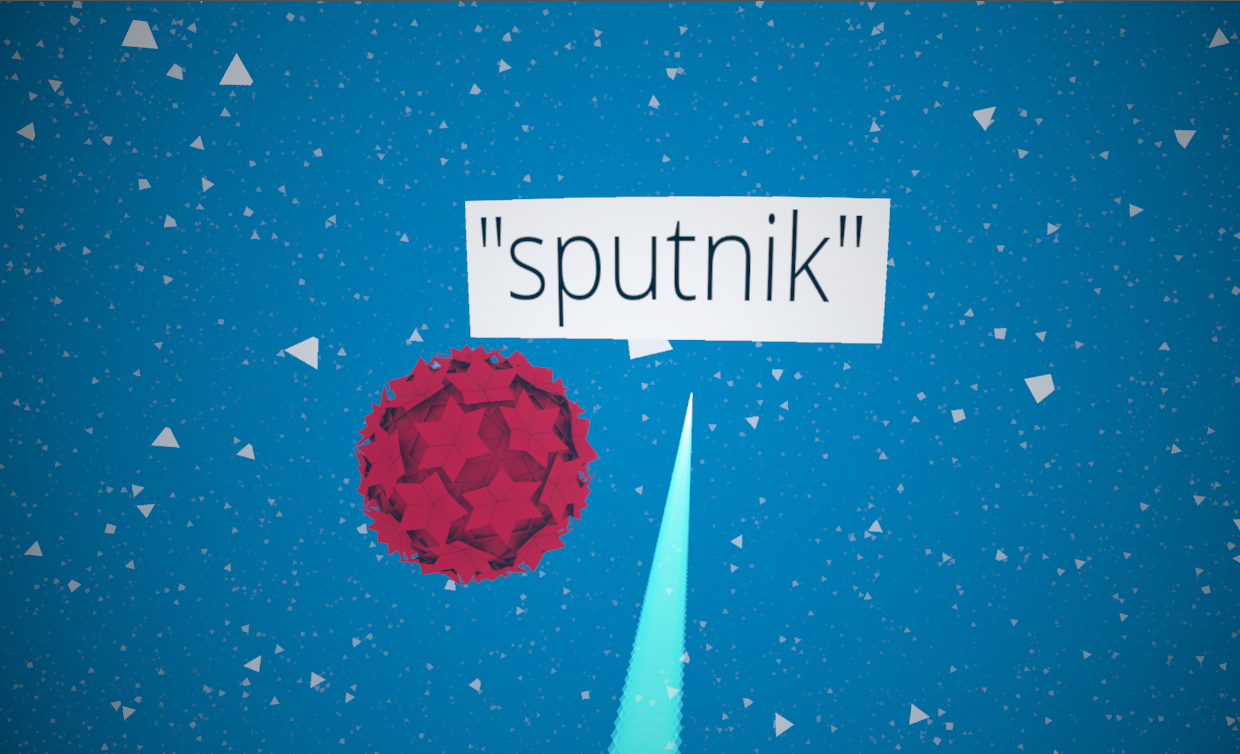
\includegraphics[width = 0.45 \columnwidth]{img/screen-shot-label}
}
\caption{(a) a group of \emph{samplers}, (b) a close-up of a sampler with its textual label}
\end{center}
\end{figure}






\section{Wiimote Input}
The Wiimote controller was chosen for its pointing functionality as well as the motion sensing capabilities, even though they haven't been used in the final project. The accompanying Nunchuck controller was also used to allow the standard analogue stick driven navigation.

The Wiimote has an built in low resolution IR camera and its feed is directly processed on chip. The feed itself is not accessible but data of up to 4 tracked IR points can be read. the Wiimote's update rate is reported to be $100Hz$ which gives an lower bound for the worst case lag of $10ms$. The used Wiimote library takes care of most of the processing and and conveniently returns the computed pointer location in relative screen coordinates.

A drastic constraint of the Wiimote's IR pointer is the relatively narrow field of view. It is very easy to leave the small sensing area resulting in no data. During the development it turned out that using the Wiimote for the tilt/pan movements of the camera can alleviate this problem a little. Users seem to intuitively try to compensate the camera rotation thus better maintaining a focus on the neutral area in the center of the screen. Without it users easily lost the focus an had troubles finding \emph{back onto the screen}.

The used library supports more than one Wiimote and the input system in Sputnik would also support multiple input devices at the same time. The option to \emph{dual wield} two Wiimotes and interact with two arcs of light simultaneously was given up in favour of the more standard analogue stick track/dolly controls to allow the users to easily navigate the scene. 









\subsection{Mapping the System}
What further distinguishes Sputnik from other projects or interfaces is the spacial component. The user cannot only drag objects to create sounds but can also change the spacial configuration of the system by moving objects. All objects that are not bound to a fixed origin (i.e. the harmonic harp) can be freely moved around and be thus allowing the system to be reconfigured at runtime. 

The tape machine and harmonic harp provide the most interesting examples for possible mappings of the system. Those two interactive objects use the physical properties of the individual objects and map them to sound parameters. This is something that is not possible with conventional hardware or software interfaces.





\section{Evaluation}
\label{sec:evaluation}
3-5 pages

Describe the evaluation according to the research questions. Describe the process and the observed results.

\subsection{What to evaluate}
\subsection{Assumptions, expected outcome}
\subsection{describe the evaluation}
\subsection{give the results}


\section{Discussion}
\label{sec:discussion}
3-5 pages

Discuss the results form the evaluation and answer the research questions. 

\begin{enumerate}
\item How can the arc of light/fishing rod metaphor be used for intuitive interaction. How does lag impact the system?
\item What meaningful mappings can be derived from the interaction with and the visualisation of the virtual scene.
\end{enumerate}

\section{Future Work}

\section{Conclusion}
0.5 pages

\section{Acknowledgements}
thank Esben, thank the participants,




\bibliographystyle{apalike}
\bibliography{related-work}

\end{document}